\subsection{WLAN - so funktioniert es}
\label{wlan}

\subsubsection{Auf dem Bot}
\label{wlan_auf_bot}
Als erstes muss das WLAN-Modul (WiPort) des ct-Bots konfiguriert werden.
Dazu verbindet man sich am Besten über die serielle Schnittstelle mit dem Modul.
(Ein spezieller USB-Adapter wird benötigt. Das rote Kabel muss beim 
Einstecken in den Roboter rechts sein.) Um in das Konfigurationsmenü zu gelangen,
muss beim Start des Bots sofort x (mehrmals, um den Zeitpunkt nicht zu verpassen)
gedrückt werden. Es erscheint folgende Ausgabe:
\begin{verbatim}
    MAC address 00204A96578C
    Software version V6.6.0.0 (080107) 
    Press Enter for Setup Mode
\end{verbatim}
Ältere Versionen haben möglicherweise andere Konfigurationsmenüs und Funktionen.
Das stellt aber im Allgemeinen kein Probelm dar. Getestet wurde auch die Version
6.3.0.0.\\

Nach dem Bestätigen der Enter-Taste wird der aktuelle
Konfigurationsstatus ausgegeben, gefolgt von einem Menü.
Mit 7 können die Einstellungen zurückgesetzt werden.
Im Menüpunkt 0 (Server) sollte darauf geachtet werden, dass Wireless verwendet wird
und dem Bot die IP 192.168.0.\textit{"'Bot-Nummer"'} zugewiesen wird.
Mit Menüpunkt 2 muss nun der Channel 2 eingestellt werden.
\begin{verbatim}
    Baudrate (9600) ? 57600
    I/F Mode (4C) ? 
    Flow (00) ? 
    Port No (10002) ? 
    ConnectMode (C0) ? CC
    Datagram Type (00) ? 01
    Send as Broadcast (N) ? 
    Remote IP Address : (000) 192.(000) 168.(000) 000.(000) 255
    Remote Port  (0) ? 10002
    Pack Cntrl  (00) ? 
    SendChar 1  (00) ? 
    SendChar 2  (00) ? 
\end{verbatim}

\noindent{Eine gültige Konfiguration könnte dann wie folgt aussehen:}
\begin{verbatim}
    *** basic parameters 
    Hardware: Ethernet TPI, WLAN 802.11bg
    Network mode: Wireless Only
    IP addr 192.168.0.9, no gateway set
    DNS Server not set

    *** Security
    SNMP is              enabled
    SNMP Community Name: public
    Telnet Setup is      enabled
    TFTP Download is     enabled
    Port 77FEh is        enabled
    Web Server is        enabled
    Web Setup is         enabled
    ECHO is              disabled
    Enhanced Password is disabled
    Port 77F0h is        enabled

    *** Channel 1
    Baudrate 9600, I/F Mode 4C, Flow 00
    Port 10001
    Connect Mode : C0
    Send '+++' in Modem Mode enabled
    Show IP addr after 'RING' enabled
    Auto increment source port disabled
    Remote IP Adr: --- none ---, Port 00000
    Disconn Mode : 00
    Flush   Mode : 00

    *** Channel 2
    Baudrate 57600, I/F Mode 4C, Flow 00
    Port 10002
    Connect Mode : CC
    Datagram Type 01
    Pack Cntrl:   00
    Remote IP Adr: 192.0.0.255, Port 10002


    *** Expert
    TCP Keepalive    : 45s
    ARP cache timeout: 600s
    CPU performance: Regular
    Monitor Mode @ bootup : enabled
    HTTP Port Number : 80
    SMTP Port Number : 25
    MTU Size: 1400
    Alternate MAC: disabled
    Ethernet connection type: auto-negotiate

    *** E-mail
    Mail server: 0.0.0.0
    Unit       : 
    Domain     : 
    Recipient 1: 
    Recipient 2: 

    - Trigger 1 
    Serial trigger input: disabled
      Channel: 1
      Match: 00,00
    Trigger input1: X
    Trigger input2: X
    Trigger input3: X
    Message : 
    Priority: L
    Min. notification interval: 1 s
    Re-notification interval  : 0 s

    - Trigger 2 
    Serial trigger input: disabled
      Channel: 1
      Match: 00,00
    Trigger input1: X
    Trigger input2: X
    Trigger input3: X
    Message : 
    Priority: L
    Min. notification interval: 1 s
    Re-notification interval  : 0 s

    - Trigger 3 
    Serial trigger input: disabled
      Channel: 1
      Match: 00,00
    Trigger input1: X
    Trigger input2: X
    Trigger input3: X
    Message : 
    Priority: L
    Min. notification interval: 1 s
    Re-notification interval  : 0 s

    *** WLAN 
    WLAN: enabled
    Topology: Ad-Hoc
    Network name: ctbot
    Country: US
    Channel: 11
    Security suite: none
    TX Data rate: 11 Mbps auto fallback
    Power management: not supported in adhoc mode
    Soft AP Roaming: N/A
\end{verbatim}

 \newpage


\noindent{\textbf{WLAN Daten Senden/Empfangen:}} \\
\\
Für genauere Infos zu bereits existierenden Funktionen sollte in der CT-Bot-Dokumentation nachgeschaut werden.\\
\\
\textbf{Senden:} Das Schreiben/Senden von Daten ist relativ einfach, da hierfür schon Funktionen zur Verfügung stehen, die genau das für einen erledigen.\\
Mit \verb|command_write(...)| können Kommandos gesendet werden, an die Optional auch Daten angehängt werden können. Dabei gibt der Payload an wie viele Bytes angehängt wurden. 
\\
\textbf{Empfangen:} Für das Empfangen gibt es die Möglichkeit, die in \textit{command.c} definierte, Funktion \verb|command_evaluate| zu erweitern. Das hat den Vorteil, dass jedes gültige Kommando, das gelesen wird, auch verarbeitet wird, solange dafür Code in \verb|command_evaluate| vorhanden ist.
Da wir aber nur unsere Kommandos verarbeiten mussten und zudem das Ziel hatten so wenig wie möglich in schon vorhandenen Dateien zu verändern, haben wir uns Hilfsfunktionen geschrieben.\\
\\
\verb|command_t* read_command()| liest ein Kommando in die schon vorhandene Variable \verb|received_command| in \textit{command.c} ein und gibt einen Zeiger darauf zurück.\\
\\
Zum Lesen wird mit der schon vorhandenen Funktion \verb|uart_data_available| geschaut, wie viele Bytes an Daten zum Lesen verfügbar sind.\\
\\
Wenn mindestens genug Daten für ein Kommando (\verb|sizeof(command_t)|) vorhanden sind, wird mit einer weiteren schon vorhandenen Funktion \verb|command_read| ein Kommando in die Puffervariable \verb|received_command| eingelesen.\\
\\
Zuletzt wird mit der von uns zu \textit{command.c} hinzugefügten Funktion \\ \verb|get_received_command| ein Zeiger auf \verb|received_command| zurückgegeben.\\
\\
\textbf{Payload-Daten auslesen:} Da nach einem Kommando noch zusätzlich Daten angehängt werden können, haben wir auch hierfür eine Funktion geschrieben.\\
\\
\verb|uint8_t* read_payload(command_t* cmd, uint8_t* buffer)| liest die angehängten Daten des übergebenen Kommandos in den übergebenen buffer.\\ Hierfür wird auf die vorhandene Funktion \verb|low_read| zurückgegriffen.

\newpage

\begin{verbatim}
typedef struct {
    uint8_t startCode;  /*!< Markiert den Beginn eines Commands */
    request_t request;  /*!< Command-ID */
    uint8_t  payload;   /*!< Bytes, die dem Kommando noch folgen */
    int16_t data_l;     /*!< Daten zum Kommando link s*/
    int16_t data_r;     /*!< Daten zum Kommando rechts */
    uint8_t seq;        /*!< Paket-Sequenznummer */
    uint8_t from;       /*!< Absender-Adresse */
    uint8_t to;         /*!< Empfaenger-Adresse */
    uint8_t CRC;        /*!< Markiert das Ende des Commands */
} PACKED command_t;

typedef struct {
#if (defined PC) && (BYTE_ORDER == BIG_ENDIAN)
    /* Bitfeld im big-endian-Fall umdrehen */
    uint8_t command;        /*!< Kommando */
    unsigned direction:1;   /*!< 0 ist Anfrage, 1 ist Antwort */
    unsigned subcommand:7;  /*!< Subkommando */
#else
    uint8_t command;        /*!< Kommando */
    unsigned subcommand:7;  /*!< Subkommando */
    unsigned direction:1;   /*!< 0 ist Anfrage, 1 ist Antwort */
#endif
} PACKED request_t;
\end{verbatim}

Damit der Bot ein WLAN-Paket als \textit{command} interpretiert, muss es einen Inhalt mit folgendem Aufbau besitzen,
wobei das \verb|direction|-Element der Struktur nicht im WLAN-Paket auftaucht:
\begin{figure}[H]
    \centering
    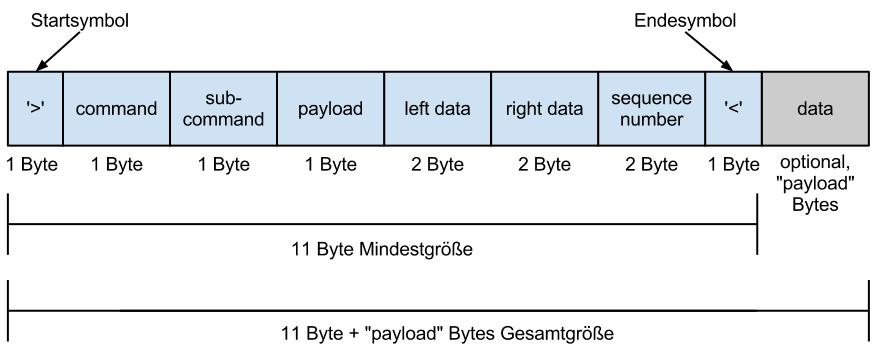
\includegraphics[scale=0.5]{pic/ctBotWlanAllgemein}
    \caption{Allgemeiner Aufbau eines \textit{commands} in einem WLAN-Paket}
    \label{ctBotWlanAllgemein}
\end{figure}


\subsubsection{Auf dem PC}
Um Daten an den Bot zu senden sind lediglich zwei Schritte erforderlich:
\begin{itemize}
    \item Zum WLAN verbinden\\
    Ist der Bot korrekt konfiguriert öffnet er ein Ad-Hoc-WLAN. Zu diesem muss man sich verbinden.
    \item Paket an den Bot senden bzw. Daten empfangen\\
    Ist man mit dem WLAN verbunden kann man einfach ein UDP-Paket mit einen speziellen Inhalt (siehe \ref{wlan_auf_bot}) an den Bot senden, so dass dieser das Paket auswerten kann.\\
    In unserem Fall sieht ein Paket folgendermaßen aus:
    \begin{figure}[H]
        \centering
        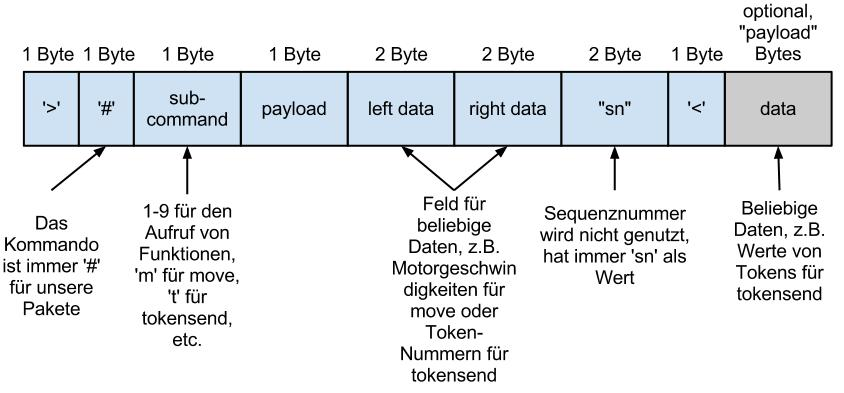
\includegraphics[scale=0.5]{pic/ctBotWlanKonkret}
        \caption{Konkreter Aufbau eines \textit{commands} für unsere Anwendung}
        \label{ctBotWlanKonkret}
    \end{figure}
    
    Hierzu kann z.B. das Tool \textit{sendip} verwendet werden. Ein Beispiel hierzu:\\
    \textit{\$ perl -e 'print "'\textgreater\#\textbackslash x02\textbackslash x06\textbackslash x03\textbackslash x11\textbackslash x02\textbackslash x02xy\textless hallo\textbackslash x00"'' \textgreater test.bin\\
    \$ sudo sendip -p ipv4 -is 192.168.0.234 -p udp -us 2000 -ud 10002 -f test.bin 192.168.0.9}\\
    Hierzu wird zunächst mit einem PERL print-Befehl ein Paket erzeugt und in eine Datei geschrieben und anschließen wird der Dateiinhalt mit \textit{sendip} an den Bot (hier 192.168.0.9) gesendet.
    (Die Paramter von links nach rechts: Protokoll IPv4, Quell-IP 192.168.0.234, Protokoll UDP, UDP-Quellport 2000, UDP-Zielport 10002, Datei (deren Inhalt gesendet werden soll) test.bin, die Ziel-IP 192.168.0.9)
    Der Grund für den Umweg über die Datei ist lediglich, dass man sich dadurch "'verlorene"' Zeichen oder kaputte Eingaben erspart, was der Fall wäre wenn man die Eingabe piped oder über eine Subshell erzeugt.
\end{itemize}
Die wesentlich einfachere Variante Pakete an den Bot zu schicken ist das Skript \verb+ctremote.py+ bzw. dessen Funktion \verb+send_cmd(...)+. Dazu siehe \ref{ctremote}.

\subsection{Zusatzaufgabe}

\subsubsection{ctremote.py - Ein Skript zur Fernsteuerung des Bots}
\label{ctremote}
Das Skript ist ein interaktives Programm, welches dem Nutzer ermöglicht Befehle einzugeben, die Aktionen auf Seiten des Bots auslösen. Dazu muss auf dem Bot das Programm laufen, welches in Abschnitt \ref{ctremote_bot} beschrieben ist.\\
Sieht der Nutzer folgenden Prompt, kann er Befehle eingeben:

\textbf{ctBot-remote \$}\\
Nachfolgend die bisher implementierten Befehle:
\begin{itemize}
    \item subcmd <subcommand>\\
    Sendet den angegebenen Subcommand <subcommand> an den Bot. Es sind bisher folgende Subcommands implementiert:
    \begin{itemize}
        \item 1 oder stand\\
        Lässt den Bot anhalten.
        \item 2 oder motte1\\
        Lässt den Bot die erste Implementierung von "'Motte"' ausführen.
        \item 3 oder kakerlake1\\
        Lässt den Bot die erste Implementierung von "'Kakerlake"' ausführen.
        \item 4 oder motte2\\
        Lässt den Bot die zweite Implementierung von "'Motte"' ausführen.
        \item 5 oder kakerlake2\\
        Lässt den Bot die zweite Implementierung von "'Kakerlake"' ausführen.
        \item 6 oder acht\\
        Lässt den Bot eine Acht fahren.
        \item 7 oder linie\\
        Lässt den Bot eine Linie entlang fahren.
    \end{itemize}
    Beispiel: \textit{subcmd motte1}
    
    Beispiel 2 : \textit{subcmd 6}
    \item move\\
    Nach Eingabe dieses Befehls ist der Bot über die Tastatur fernsteuerbar. Die Tastenbelegung dafür ist wie folgt:
    \begin{itemize}
        \item \textbf{W} Vorwärts fahren.
        \item \textbf{S} Rückwärts fahren.
        \item \textbf{A} Nach links drehen.
        \item \textbf{D} Nach rechts drehen.
        \item \textbf{E} Anhalten.
        \item \textbf{Q} Beendet den move-Befehl und kehrt zur Befehlseingabe zurück.
    \end{itemize}
    \item tokensend <tokenfile>\\
    Dieser Befehl sendet ein sogenanntes Tokenfile an den Bot. So ein Tokenfile ist eine Textdatei mit folgendem Aufbau:
    \begin{verbatim}
    Token Value
    \end{verbatim}
    Z.B.:
    \begin{verbatim}
        5 while
        7 a
        45 =
        7 b
    \end{verbatim}
    Dabei handelt es sich um Tokens (samt zugehöriger Werte), die ein selbstgeschriebener Scanner für die Programmiersprache "'Fun"' erzeugt hat. Es wurde ein "'Fun"'-Compiler bzw. Interpreter auf den Bot portiert, der im Rahmen der Vorlesung Compilerbau erstellt wurde. Die Trennung erfolgte zwischen Scanner (läuft auf dem PC) und Parser/Codegenerierung/Interpretierung (läuft auf dem Bot) und die kleinst mögliche Menge an Daten übertragen zu müssen. Der Bot ist nun mit "'Fun"'-Code steuerbar/programmierbar. So muss man den Bot nicht immer neu flashen sondern kann ihn in "'Fun"' programmieren und die Programme einfach per WLAN übertragen.
    \item get <what>\\
    Zeigt einem den aktuellen Wert von <what> an. Dabei kann <what> momentan \textit{botip} (also die IP des zu steuernden Bots) oder \textit{port} (also der UDP-Port, über den kommuniziert wird) sein.
    
    Beispiel: \textit{get botip}
    \item set <what> <value>\\
    Setzt den Wert von <what> auf <value>. Hierbei kann <what> wieder \textit{botip} oder \textit{port} sein.
    
    Beispiel: \textit{set botip 192.168.0.9}
    \item help\\
    Gibt einen kurze Übersicht aller Befehle mit einer kurzen Beschreibung aus.
    \item help <cmd>\\
    Gibt einen detaillierten Hilfetext zum angegebenen Befehl <cmd> aus.
    
    Beispiel: \textit{help subcmd}
    \item exit\\
    Beendet das Skript.
    \item quit\\
    Beendet das Skript.
\end{itemize}
Die Tastenkombination \textit{STRG+C} wird von dem Skript abgefangen und sendet dem Bot sofort den Befehl zum Anhalten, beendet das Skript jedoch nicht. Um das Skript zu beenden muss einer der oben beschrieben Befehle \textit{quit} oder \textit{exit} verwendet werden.

\subsubsection{Aufbau von ctremote.py}
Das Skript besteht intern aus folgenden Funktionen:

\begin{itemize}
    \item \verb+help(cmd="")+\\
    Die Funktion bekommt einen optionalen Parameter \textit{cmd}. Wird kein Parameter übergeben, gibt die Funktion einen allgemeinen Hilfetext aus. Wird jedoch ein Befehl als Parameter übergeben, gibt die Funktion eine, für den übergebenen Befehl, passende Hilfe aus.
    \item \verb+openSocket()+\\
    Die Funktion öffnet einen neuen UDP-Socket mit IP und Port der aktuellen Konfiguration. (IP und Port entweder wie im Skript selbst hinterlegt oder mit dem \textit{set}-Befehl (siehe \ref{ctremote}) gesetzt.)
    \item \verb+send_cmd(subcmd,ldata="ld",rdata="rd",payload="\x00",data="")+\\
    Diese Funktion ist dafür zuständig ein Paket nach Norm des Bots (siehe \ref{wlan_auf_bot}) zusammenzubauen und schließlich an ihn zu senden.
    Der einzig zwingend nötige Parameter ist der Subcommand \textit{subcmd} (1 Byte), welcher dem Bot die auszuführende Aktion mitteilt.
    Optionale Parameter sind \textit{ldata} (2Byte) und \textit{rdata} (2 Byte), welche z.B. als Parameter für den Subcommand genutzt werden können, sowie \textit{payload} (1 Byte, Größe von \textit{data}) und \textit{data} (bis zu 255 Byte), welche genutzt werden können, wenn man zusätzliche Daten an den Bot senden will.
    Die Größe der Parameter ist dabei genau einzuhalten.
    \item \verb+recv()+\\
    Diese Funktion läuft während der gesamten Ausführung des Skripts als Thread und ist dafür zuständig Daten vom Bot zu empfangen und zu verarbeiten.
    \item \verb+user_input_eval(usrin)+\\
    Diese Funktion ist dafür zuständig die Eingaben des Nutzers zu interpretieren und die entsprechenden Aktionen durchzuführen, indem sie die anderen Funktionen des Skripts aufruft.
    Der zwingend anzugebende Paramter \textit{usrin} ist dabei die Eingabe des Nutzers.
    \item \verb+move()+\\
    In dieser Funktion läuft eine Schleife, welche dauerhaft die Tastatureingaben einliest und entsprechend der Eingabe den Bot fahren lässt (wozu sie intern \verb+send_cmd+ nutzt). Die Schleife wird erst duch drücken der Taste Q beendet.
    \item \verb+tokensend(infile="")+\\
    Diese Funktion liest ein sog. Tokenfile zeilenweise ein und baut aus jeder Zeile ein WLAN-Paket bzw. \textit{command} zusammen, welches an den Bot geschickt wird. Jedes Paket enthält den jeweiligen Token in \textit{ldata} und \textit{rdata} (zweimal aus Redundanzgründen, also zu Überprüfung der korrekten Übertragung) sowie den Value des Tokens in \textit{data}. Um den Beginn einer Tokenfile-Übertragung zu signalisieren, wird zunächst ein Paket geschickt, welchen lediglich den \textit{subcommand} "'\textit{t}"' (und sonst nur Standardwerte) enthält, versendet. Das Ende einer Übertragung wird durch ein "'0"'-Token signalisiert, welches am Ende jedes Tokenfiles steht.
%Paket signalisiert, in dem \textit{ldata} und \textit{rdata} beide auf \verb+0xffff+ gesetzt sind.
\end{itemize}


\subsubsection{Programm auf dem Bot}
\label{ctremote_bot}
Die Auswertung der Befehle die per WLAN empfangen werden, geschiet im wesentlichen
in einem \textit{swicht-case} Block. Die einzelnen Fälle werden durch das Byte \\
\verb+cmd->request.subcommand+ auseinander gehalten. Folgende Fälle wurden
implementiert:
\begin{itemize}
    \item Funktion Stand: Der Bot bleibt stehen.
    \item Funktion Motte 1: Die erste Implementierung des Motte-Verhaltens.
    \item Funktion Motte 2: Die zweite Implementierung des Motte-Verhaltens. 
    \item Funktion Kakerlake 1: Die erste Implementierung des Kakerlake-Verhaltens.
    \item Funktion Kakerlake 2: Die zweite Implementierung des Kakerlanke-Verhaltens.
    \item Funktion Acht: Der Bot fährt eine Acht. Diese kann mit der Fernbedieung justiert werden.
    \item Funktion Linie: Der Bot folgt einer schwarzen Linie.
    \item Funktion Move: Der Bot kann vom Computer aus ferngesteuert werden.
        Die Geschwindigkeit für das linke bzw. rechte Rad werden in dem WLAN-Paket übertragen.
    \item Funktion Token empfangen: Liest Token über Wlan und baut einen AST für den Interpreter daraus.
\end{itemize}

\subsubsection{WLAN Flashen}
\label{wlan-flash}

\noindent{\textbf{Idee}}
\\
\\
Die Idee den Bot über Wlan flashen  zu können kam uns weil es einfach zu lange dauert schnell mal was zu probieren oder Parameter im Programm anzupassen.
\\
\\
\noindent{\textbf{Implementierung}}
\\
\\
Die Aktuelle Implementierung ist mehr ein "proof of concept" da es viel Zeit gekostet hat bis zum ersten funktionierenden Beispiel auf dem Bot. 
Da wir parallel zu Mobile Roboter auch Compilerbau besucht haben, war es nur logisch den dort entworfenen Compiler/Interpreter auf den Bot zu portieren.
Hier ist eine List der Probleme die dabei auftraten und die >Aktuelle< Lösung.
Langfristige Lösungen werden danach aufgeführt.
\\
\begin{itemize}
	\item 	\textbf{Problem:} Lex ist nicht portierbar ohne den generierten Code anzupassen. \\
		\textbf{Lösung:} Trennung von Scanner(PC) und Parser/Interpreter(BOT).

	\item 	\textbf{Problem:} Begrenzter Speicher auf den Bot. \\
		\textbf{Lösung:} Löschen von unnötigen Dateien von Vorgängergruppen.
	
	\item 	\textbf{Problem:} Übertragungsfehler im WLAN. \\
		\textbf{Lösung:} Erneutes senden der Tokens.
\end{itemize}


\noindent{\textbf{Zukunft}}
\\
\\
Die Idee kann natürlich in alle Richtungen ausgebaut und optimiert werden.
Angefangen damit das als Grundlage eine verlässliche Übertragung für den Bot implementiert werden muss.
Zum Punkt Speicherplatz und Effizienz auf dem Bot wäre es Sinnvoll nur einen minimalen Interpreter/VM
 auf dem Bot zu haben und stat Tokens Bytecode/Instructions zu übertragen.
  Die Programmiersprache sollte auch angepasst und erweitert werden um die volle funktionallität des Bots nutzen zu können und flexibler zu sein.
